\documentclass[a4paper,11pt]{article}

% \usepackage[colorlinks,linkcolor=blue,anchorcolor=blue,citecolor=blue]{hyperref}

% \usepackage[colorlinks, linkcolor=blue, anchorcolor=blue, citecolor=blue, urlcolor=blue]{hyperref}

\usepackage{jinstpub} % for details on the use of the package, please see the JINST-author-manual
\usepackage{lineno}




% \usepackage{authblk}
\linenumbers

% Proceedings/Special Issues
% Please note that this macro will be edited in production 
%% \proceeding{N$^{\text{th}}$ Workshop on X\\
%% When\\
%% Where}
\renewcommand{\thefootnote}{\fnsymbol{footnote}}


\title{\boldmath Single event effects in the HCCStar ASICs for ITk strip upgrade}

% Collaborations

%% [A] If main author
%% \collaboration{\includegraphics[height=17mm]{collabroation-logo}\\[6pt]
%%  XXX collaboration}

%% or
%% [B] If "on behalf of"
%% \collaboration[c]{on behalf of XXX collaboration}


% Authors
% Please note that in JINST a corresponding author is required alongside with their e-mail addres
% The "\note" macro will give a warning: "Ignoring empty anchor...", you can safely ignore it.

%% [A] simple case: 2 authors, same institution
%% \author[1]{A. Uthor\note{Corresponding author.}}
%% \author{and A. Nother Author}
%% \affiliation{Institution,\\Address, Country}

%% or, e.g.
%% [B] more complex case: 4 authors, 3 institutions, 2 footnotes
% \author[a,b]{F. Irst,\note{Corresponding author.}}
% \author[c]{S. Econd,}
% \author[a]{T. Hird\note{Also at Some University.}}
% \author[c]{and Fourth}
% \affiliation[a]{Institution_1,\\Address, Country\\}
% \affiliation[b]{Institution_2,\\Address, Country\\}
% \affiliation[c]{Institution_3,\\Address, Country}

\author[a,b,*]{Shaogang Peng,\note{Corresponding author.}}
\author[c]{Jeff Dandoy,}
\author[d]{Bruce Gallop,}
\author[e]{Hantao Jing,}
\author[f]{Jaya John John,}
\author[g]{Paul Keener,}
\author[f]{Pedro Leitao,}
\author[e]{Qiang Li,}
\author[b,h,*]{Weiguo Lu,}
\author[g]{Godwin Mayers,}
\author[g]{Mitch Newcomer,}
\author[d]{Peter Phillips,}
\author[e]{Zhixin Tan,}
\author[i]{Matt Warren,}
\author[a]{Yan Zhou}


\affiliation[a]{Department of Physics, Tsinghua University,\\Haidian District, Beijing, China}
\affiliation[b]{Institute of High Energy Physics, Chinese Academy of Sciences,\\19B Yuquan Road, Shijingshan District, Beijing, China}
\affiliation[c]{Carleton University,\\Ontario, Canada}
\affiliation[d]{Particle Physics Department, STFC Rutherford Appleton Laboratory, \\Harwell Science and Innovation Campus, Didcot, United Kingdom}
\affiliation[e]{Spallation Neutron Source Science Center, \\Dongguan, China}
\affiliation[f]{Experimental Physics Department, CERN, \\Geneva, Switzerland}
\affiliation[g]{Department of Physics and Astronomy, University of Pennsylvania, \\South 33rd Street, Philadelphia, U.S.A.}
\affiliation[h]{State Key Laboratory of Particle Detection and Electronics, \\19B Yuquan Road, Shijingshan District, Beijing, China}
\affiliation[i]{Department of Physics and Astronomy, University College London, \\Gower Street, London, United Kingdom}


% E-mail addresses: only for the corresponding author
\emailAdd{shaogang.peng@cern.ch, weiguo.lu@cern.ch}

\abstract{Triple Modular Redundancy (TMR) technology has been made in the design of the HCCStar to reduce digital state changes and ensure reliable operation.\ We tested the effectiveness of the protection by placing HCCStar chips
in a proton beam.\ We
studied corrected bit flips in registers and actual single event effects in the LCB and LP paths under
different proton energies.\ Our estimate is that there will
be $\mathcal{O}(10)$ corrected bit flips per HCCStar bit per year at the HL-LHC.\ The total ionizing
dose effect was monitored as well during the testbeam.}

\keywords{HL-LHC, CSNS, Proton, HCC, SEE, ASICs}

% \arxivnumber{1234.56789} % Only if you have one





\begin{document}
\maketitle
\flushbottom

\section{Introduction} 
\label{sec:intro}

To prepare for the High-Luminosity upgrade of the Large Hadron Collider (HL-LHC), the ATLAS experiment is replacing its Inner Detector with the all-silicon Inner Tracker (ITk), which includes the innermost pixel layers and the outermost strip layers~\cite{collaboration2008atlas}.\ The ITk is specifically engineered to withstand high radiation levels and operate at faster readout speeds, which are critical to manage the increased luminosity expected at the HL-LHC~\cite{dandoy2023irradiation}. 

The ABCStar, a latest version of the ATLAS Binary Chip (ABC), has undergone extensive testing to assess its radiation resistance~\cite{basso2022starry, peng2024single}.\ The Hybrid Controller Chip (HCC) plays a pivotal role by transmitting clock and control signals to the ABC and receiving data back from it.\ We tested the latest version of the HCC, HCCStar Version 1.\ In the worst-case scenario, these ASICs are anticipated to receive a maximum total radiation dose of up to 50 MRad~\cite{atlas2017technical}. 

% the results regarding the Autonomous Monitoring and Control Chip (AMAC) will be provided later, all of which are integral to the ITk's data readout, monitoring, and control systems.\ 

% Meanwhile, the AMAC is designed to monitor essential parameters such as voltage, current, and temperature within the ITk strip modules.\ Additionally, the AMAC can control various functions to ensure optimal operation under different conditions.\ 

It is essential to conduct extensive testing to ensure that the HCC
will operate reliably in the high-radiation environment of the HL-LHC.\ HCCs have undergone rigorous tests for radiation tolerance using gamma irradiation and heavy ions~\cite{dandoy2023irradiation, dandoy2023testing}.\ We have performed the irradiation of HCC with proton beams, adjusting the beam energy to explore the relationship between bit flip and energy.\ Through this beam testing, we aim to perform a comprehensive analysis of the HCC.

Single Event Effects (SEEs) are phenomena that occur when particles ionize materials as they pass through them and cause an observable change.\ Specifically, two types of SEEs to which the HCC is particularly susceptible are Single Event Upsets (SEUs) and Single Event Transients (SETs).\ SEUs occur when the charge deposited by an ionizing particle affects both dynamic and static memory registers storing logic states~\cite{karnik2004characterization}.\ On the other hand, SETs occur when a transient charge pulse generated by an ionizing event leads to temporal disorder of the signal~\cite{ferlet2013single}.\ The SEE protection mechanism built into ASIC designs must undergo thorough testing, which is achieved by exposing the ASICs to test beams in specialized laboratory environments and closely monitoring their operational performance.\ During the delivery of these beams, SEEs are anticipated to take place and are expected to be mitigated by the ASICs' protective mechanisms.\ Distinguishing between SEUs and SETs can be challenging during these beam tests; however, simulations have confirmed that the strategies adopted in the ASIC design protect against both types of events~\cite{ashmanskas2023verification}.

% To ensure robustness against these effects, ASIC designs incorporate specific protection mechanisms against SEEs, which must be thoroughly tested. This testing is typically conducted by placing the ASICs within the path of test beams at specialized laboratory facilities. These beams simulate the natural particle environment and help assess the ASICs' ability to handle SEEs. Throughout the beam delivery, it is expected that SEEs will occur, and the effectiveness of the ASIC designs in correcting these errors can be evaluated.

% However, differentiating between SEUs and SETs in beam tests can be challenging due to the transient nature of these events and their similar manifestations in circuit behavior. Nonetheless, simulations have demonstrated that the protective measures implemented in the ASIC designs are capable of guarding against both types of events, ensuring the stability and reliability of the system under conditions likely to produce SEEs.

% The ASIC design uses triplication and majority voting mechanisms to enhance the protection of the HCC chips against SEEs.\ In this setup, most of the logic in the chips is triplicated, meaning that three identical copies of each logic component are created.\ These copies are compared, and a majority vote is used to determine the correct output value.\ The voting circuits themselves are also triplicated to further ensure reliability.\ Due to space constraints on the HCC chip, certain components are not triplicated, including inputs, outputs, and the large memory sections dedicated to physics data storage.\ Additionally, deglitchers on the digital input pads provide extra protection against SETs by filtering out brief, unintended signal changes.\ Flip-flops are spaced at a minimum distance of 15 $um$. This spacing reduces the likelihood that one particle would affect multiple cells simultaneously~\cite{dandoy2023irradiation}.

% The purpose of beam testing is to assess whether these protective measures are sufficient to safeguard the ASICs from SEEs under real operational conditions, ensuring that HCC chips can reliably perform in the high-radiation environment of the HL-LHC.

\section{HCC chip}

The HCC ASIC serves as the digital interface for the ITk Strips hybrids in both the endcap and barrel.\ It receives a 160 MHz clock signal and two 160 Mbps control signals over a multidrop line originating from the End of Substructure card (EOS).\ The HCC decodes the control dataand generates a 40 MHz bunch crossing clock by dividing the 160 MHz clock and setting its phase from the control data framing.\ The HCC distributes this clock along with relevant control signals to between 6 and 11 ABCStar ASICs on the hybrid via shared multidrop lines.\ These control signals include triggers, event data readout requests, register read and write commands, test pulse generation, and reset signals.

\begin{figure}[htbp]
\centering
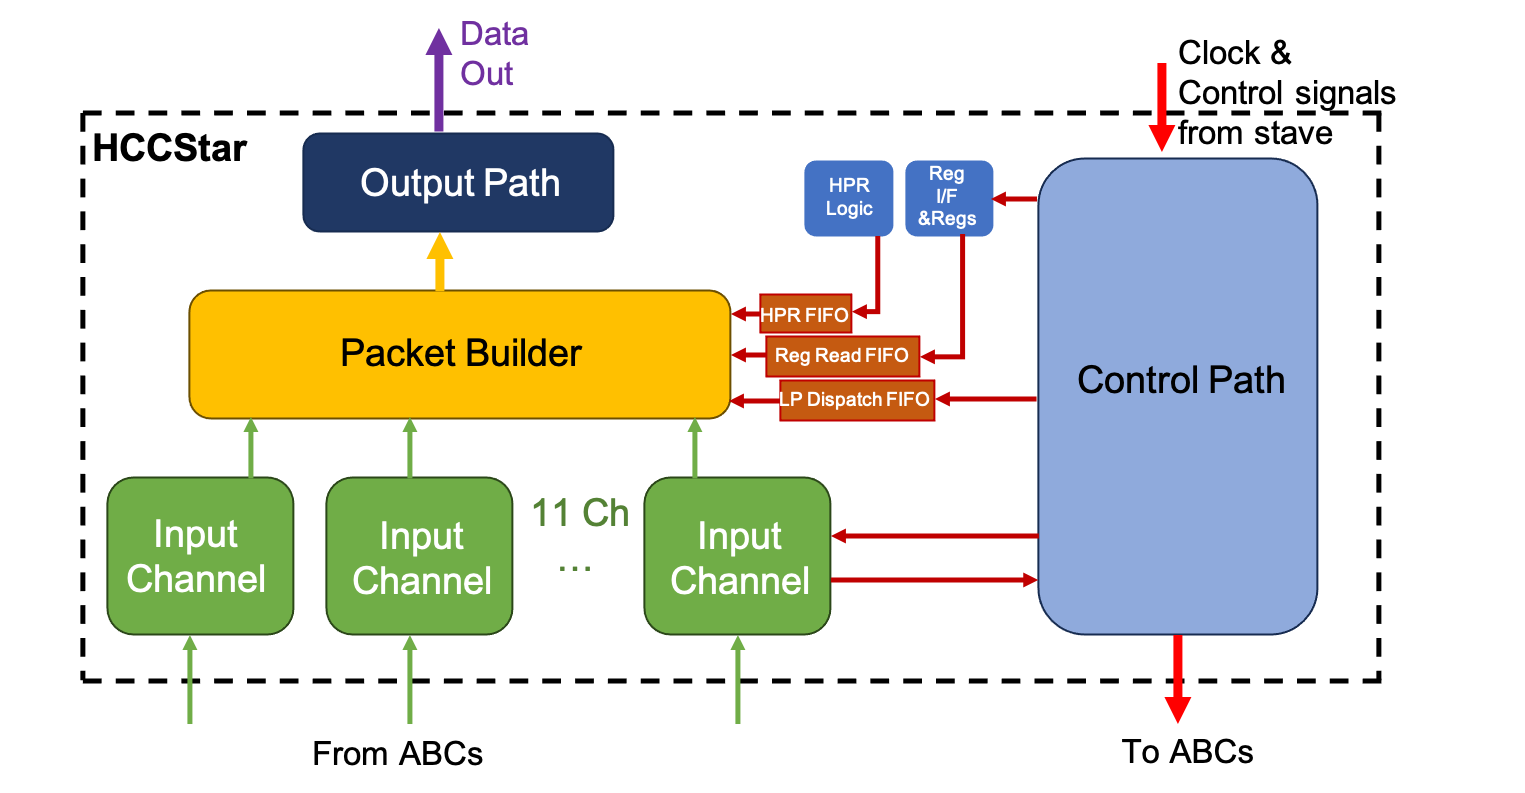
\includegraphics[width=1.0\textwidth]{images/diagram1.png}
\caption{HCC Top Level Block Diagram.\label{fig:1}}
\end{figure}

The top level block diagram of the HCC is illustrated in Figure ~\ref{fig:1}.\ System clock and control signals enter the HCC from the stave and pass through the Control Path, where these signals are processed and modified as necessary for the ABCStar ASICs on the hybrid.\ Data from the ABCStar ASICs on the hybrid is received by the HCC’s Input Channels, with one dedicated channel for each ABCStar.\ The Packet Builder then collects data from the various Input Channels, combines them into event fragments, serializes the combined data, and sends the resulting packets across the bus tape to the EOS.

\section{CSNS irradiation}

In September 2023, tests were performed at the Associated Proton Experimental Platform at CSNS~\cite{zhang2024radiation} in China, where two HCCs were simultaneously exposed to 20 \textasciitilde{} 80 MeV protons.\ 
the flux were from $4.64 \times 10^{7}$  to $5.32 \times 10^{9}$ p/cm$^{2}$/s, the total fluence were about $7.06 \times 10^{14}$ p/cm$^{2}$, and the total dose was about 24 Mrad.\ To minimize the impact of SEE on the circuits as much as possible, two HCC setups are placed in the lead bricks bunker, excluding the single-chip board.\ Over a 37 hours beam time, the ASICs experienced a total fluence equivalent to approximately 48\% of the HL-LHC's expected lifetime.

The HCC chips utilize the Inner Tracker Strips DAQ (ITSDAQ) software for data readout.\ The ITSDAQ firmware is loaded on the Nexys Video FPGA board, enabling monitoring of both register and physics data.\ However, the buffers that receive data from the ABCs do not protect the physics data path from SEEs, except for metadata like L0tag, BCID, and the last cluster bit which are secured.

When Triple Modular Redundancy (TMR) is enabled, any changes in the data bits are detected by the triple modular circuit.\ This setup compares the altered bits with two other circuits to decide whether to retain the changes.\ Following this comparison, the bits are reset, ensuring they do not disrupt the ASICs’ normal functions.\ The corrected bits in this context are referred to as Corrected Bit Flips (CBFs).\ During our tests, we observed numerous CBFs and aimed to prevent actual SEEs because of design considerations.\ Despite these precautions, we noted that SEEs still occurred as the energy increased.

Conversely, in circuits lacking TMR protection, actual SEEs are observed directly, without any CBFs.\ These SEEs can happen in both the registers and the physics data path, impacting components like the L0A/CMD/BCR (LCB) or Low Priority readout request (LP) lines.\ To specifically address SEEs that occur in registers (ASIR), dedicated registers (address 0, 1) count the occurrences in other registers.\ The LCB line transmits messages to the HCC, while the LP line relays the trigger decision from the HCC to the ABCs.\ Although SEEs in the LP path (ASLP) are detected, no SEEs have been observed in the LCB data line during our testing.





\section{Results}
For the registers, we need to normalize according to the number of bits monitored for each individual chip.\ The calculation formula for the cross section of SEEs in the registers is shown as: 

\begin{equation}
\label{eq:x}
\begin{aligned}
\sigma_{reg} &= \frac{\#\text{Bit Flips (CBFs or actual SEEs)}}{\#\text{fluence} \cdot \#\text{bits monitored}} \,,
\qquad
% y = 2 \,,
% \\
% z &= 3 \,.
\end{aligned}
\end{equation}
we monitored a total of 16 registers $\times$ 32 bits/register = 512 bits.\ When calculating the cross section for physics data, the formula is as follows:

\begin{equation}
\label{eq:x1}
\begin{aligned}
\sigma_{LCB\ or\ LP} &= \frac{\#\text{Bit Flips (actual SEEs)}}{\#\text{fluence}} \,,
\qquad
% y = 2 \,,
% \\
% z &= 3 \,.
\end{aligned}
\end{equation}
in the case of zero measured bit flip, 95\% upper confidence bound is calculated by assuming 3 bit flips, we assume that the observed bit flips follow Poisson statistics distribution.

The process of CBFs is continuous, leading to a difference in the fluence of CBFs observed in registers compared to those detected in the data path.\ As we are able to monitor bit flips that are being continuously corrected when accessing the SEE registers.\ In contrast, sensitivity to SEEs within the data path is limited to the short period during data readout.

To test the effectiveness of TMR, we placed two chips simultaneously in a 70 MeV beam and performed irradiation tests with and without triplication enabled, the irradiation time was kept the same for both chips.\ The cumulative cross section for each chip is shown in Table~\ref{tab:t1}.

\begin{table}[htbp]
\centering
\caption{Cumulative bit flip cross sections from CSNS proton data.\label{tab:t1}}
\smallskip
\small{
\setlength{\tabcolsep}{2mm}
\begin{tabular}{l|c|c|c|c|c|c|c}
\hline

Chip & 3 clocks? & CBFs &  $\sigma_{CBFs}$ [cm$^{2}$/p/bit] & ASIR & $\sigma_{ASIR}$ [cm$^{2}$/p/bit] & ASLP & $\sigma_{ASLP}$ [cm$^{2}$/p] \\
\hline
    &      & 445/ & 1.02$\times$10$^{-13}$/  &    0/ & 6.89$\times$10$^{-16}$/ &  0/ & 3.53$\times$10$^{-13}$/\\
154 & Yes/ &  0/  & 9.99$\times$10$^{-16}$/  & 7953/ &      
    2.65$\times$10$^{-12}$/ & 32/ & 5.46$\times$10$^{-12}$/    \\

\cline{1-1}
\cline{3-8}

152 & No/ & 450/ & 1.03$\times$10$^{-13}$/ &   0/ & 6.89$\times$10$^{-16}$/      & 13/ & 1.53$\times$10$^{-12}$/\\
    &     &  0/  & 6.52$\times$10$^{-16}$/ & 168/ & 3.65$\times$10$^{-14}$/
    & 15/ & 1.67$\times$10$^{-12}$/\\

% Chip&y&x and y\\
% \hline
% a & b & a and b\\
% 1 & 2 & 1 and 2\\
% $\alpha$ & $\beta$ & $\alpha$ and $\beta$\\

\hline
\end{tabular}}
\end{table}

"3 clocks" represents enabling the triplication, from the table, we can see that there are no CBFs without triplication, moreover, the cross section when the triplication is not enabled is several orders of magnitude larger than when it is enabled, which means TMR works as expected.\ Additionally, the cross section of CBFs is approximately 10$^{-13}$ cm$^{2}$/p/bit, which is consistent with the results from TRIUMF~\cite{dandoy2023irradiation}.

We also studied the cross section with beam energy varying from 20 MeV to 80 MeV.\ As seen in Figure ~\ref{fig:2}, the
number of actual SEEs generally tends to increase as the energy increases.



% \begin{figure}[htbp]
% \centering
% 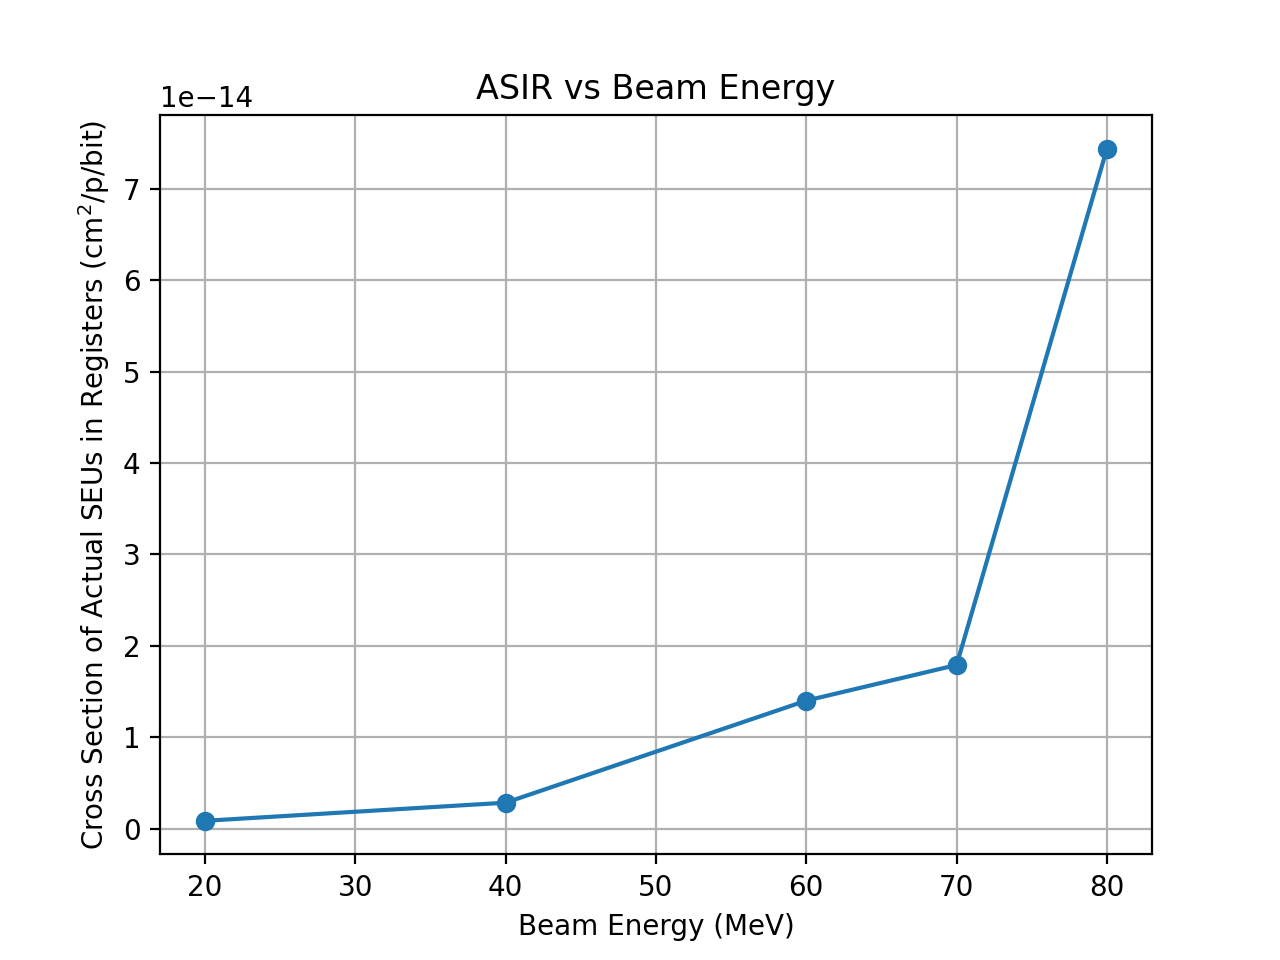
\includegraphics[width=.479\textwidth]{images/Figure_2.png}
% \quad
% 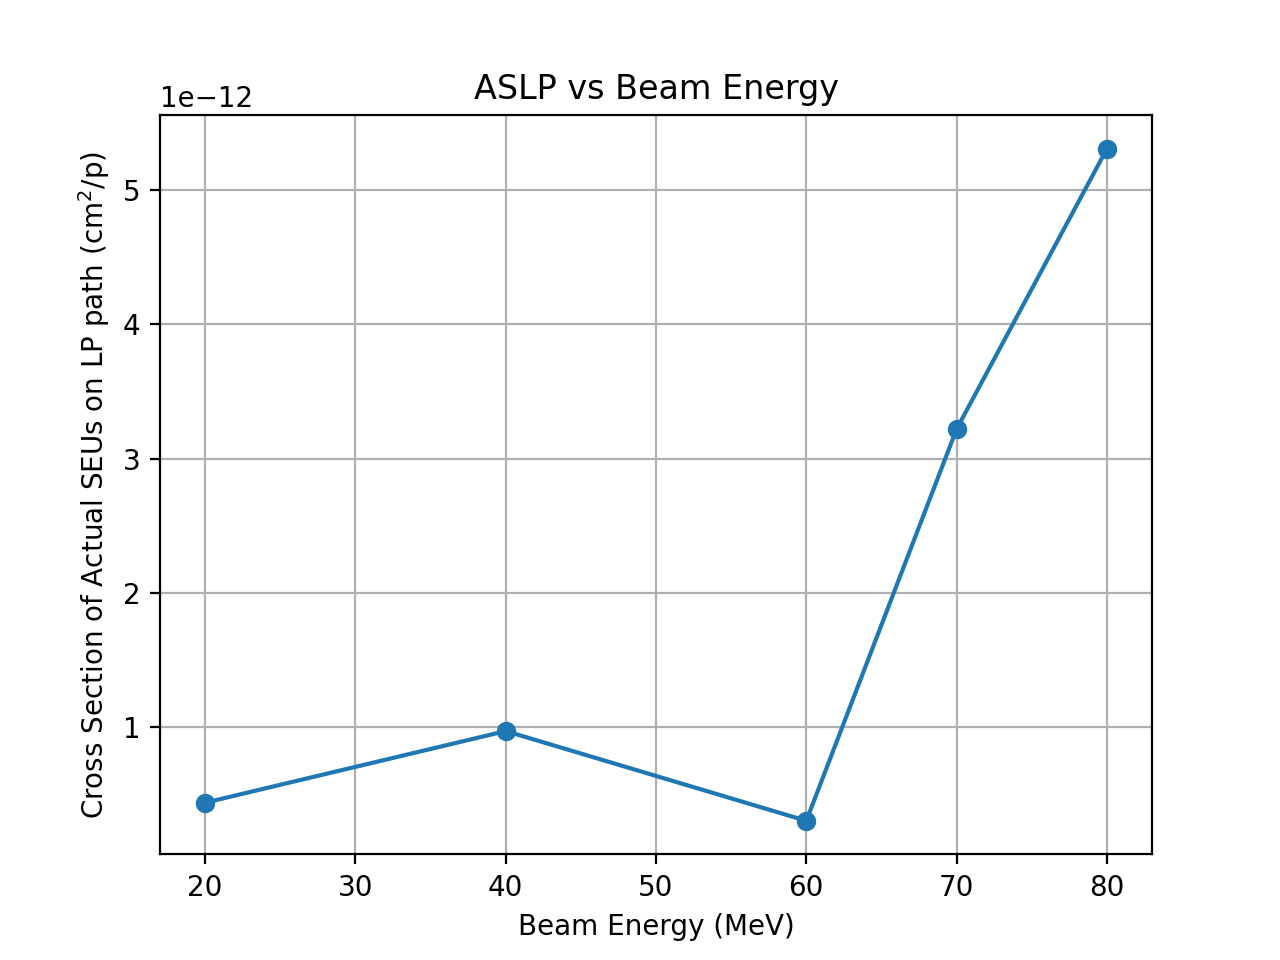
\includegraphics[width=.479\textwidth]{images/Figure_3.png}
% \caption{The cross section of actual SEEs measured at the CSNS proton testbeam as a function of beam energy.\label{fig:2}}
% \end{figure}


\begin{figure}[htbp]
\centering
\begin{minipage}{.51\textwidth}
  \centering
  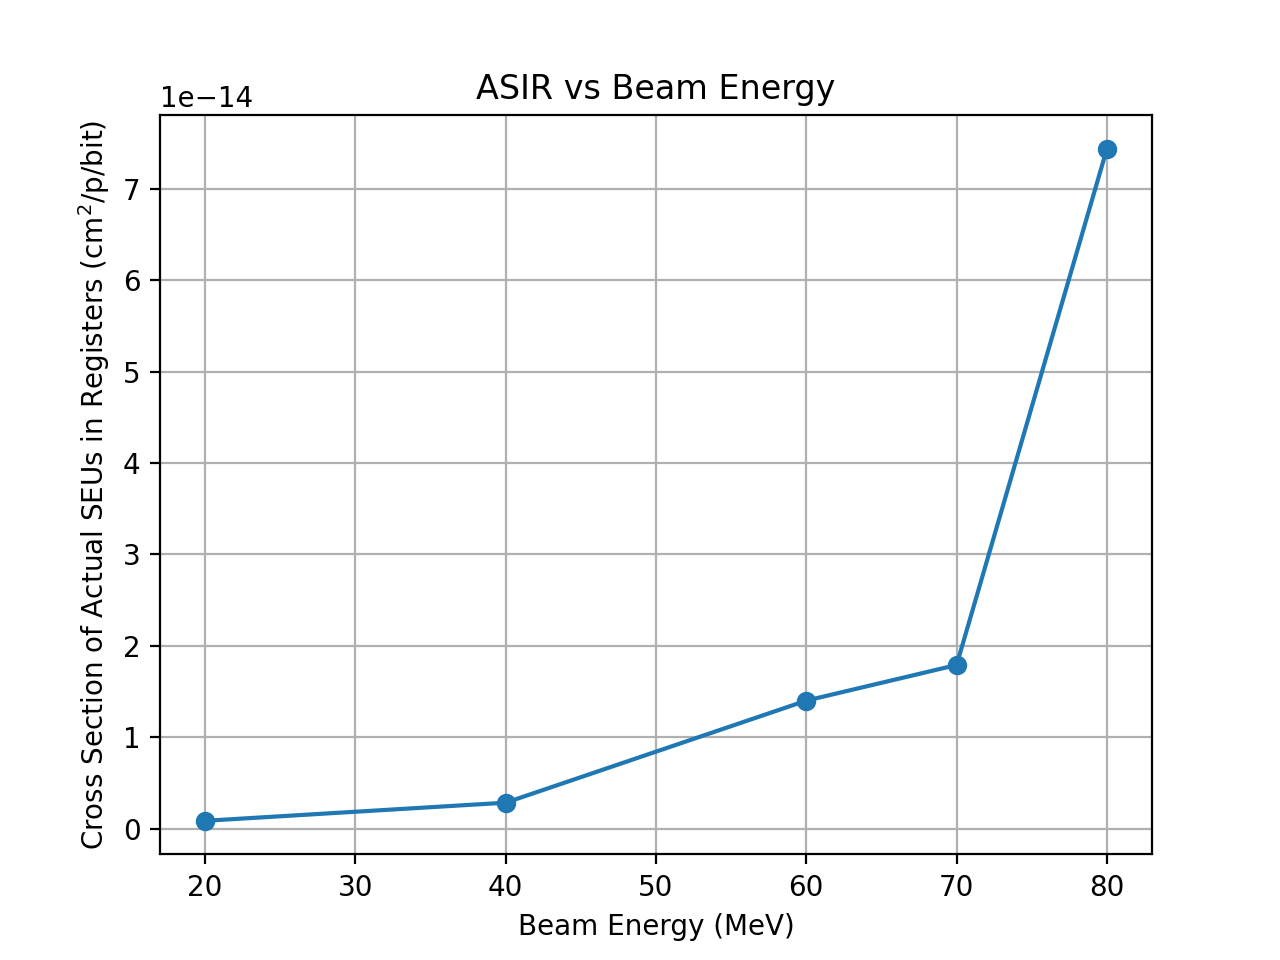
\includegraphics[width=\linewidth]{images/Figure_2.png}
\end{minipage}%
\begin{minipage}{.51\textwidth}
  \centering
  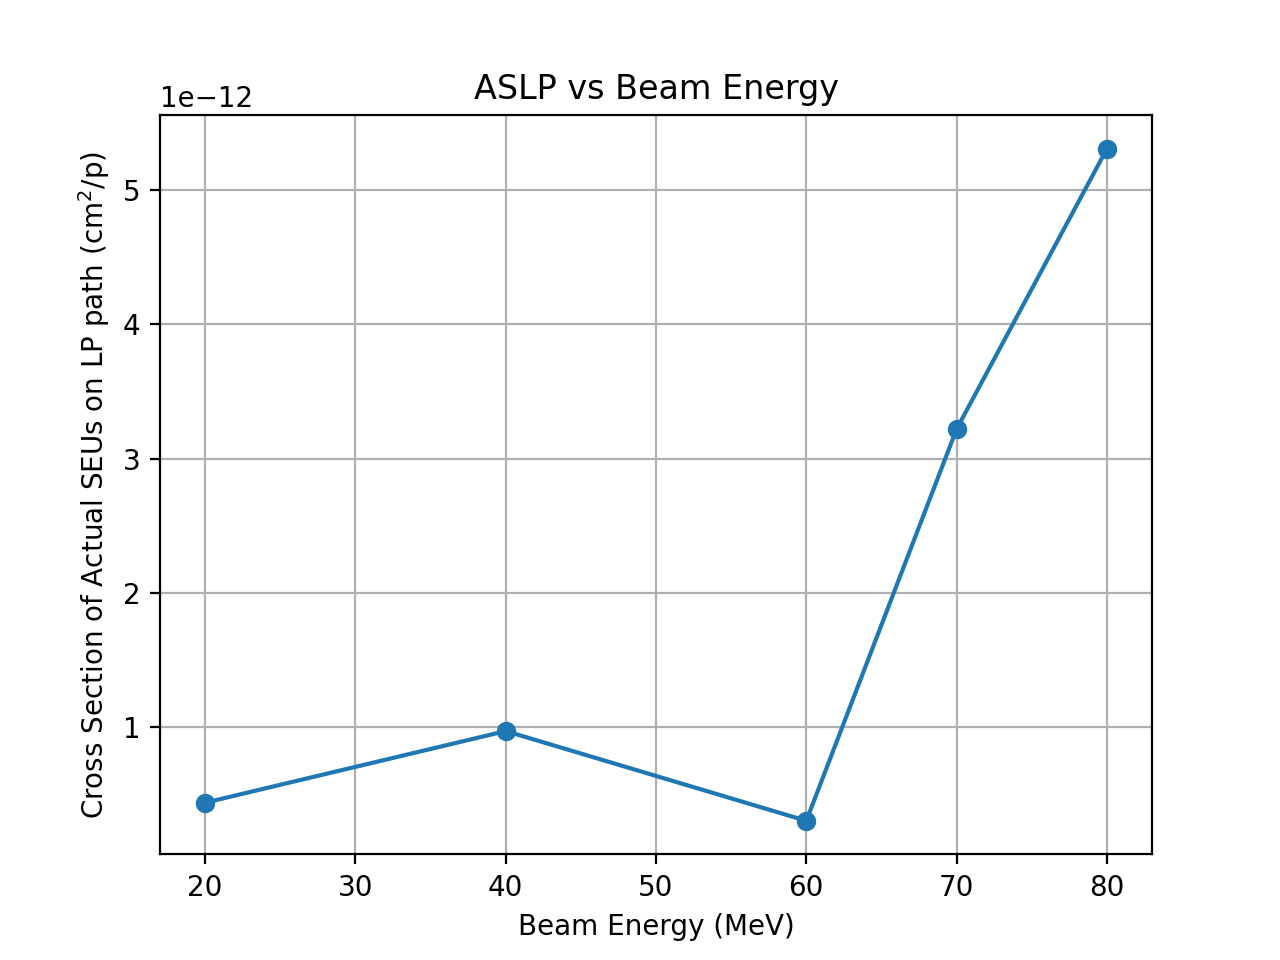
\includegraphics[width=\linewidth]{images/Figure_3.png}
\end{minipage}
\caption{The cross section of actual SEEs in registers or LP path measured at the CSNS proton testbeam as a function of beam energy.\label{fig:2}}

\end{figure}

We can calculate the rate of CBFs, Rate$_{\text{CBFs}}$ is given by:

\begin{equation}
\label{eq:x}
\begin{aligned}
\text{Rate}_{\text{CBFs}} 
  &= \Phi_{\text{hadrons}} \cdot \frac{\sigma_{\text{SEE}}}{\text{chip}} \cdot \frac{10^{7} \text{s} }{\text{year}} \\
  &= \mathcal{O}(10^{7}) \frac{\text{hadrons}}{\text{cm}^{2} \cdot \text{s}} \cdot \frac{\sigma_{\text{SEE}}}{\text{chip}} \cdot \frac{10^{7} \text{s} }{\text{year}} \\
  &= \mathcal{O}(10^{7}) \frac{\text{hadrons}}{\text{cm}^{2} \cdot \text{s}} \cdot \mathcal{O}(10^{-13}) \frac{\text{cm}^{2}}{\text{bit}} \cdot \frac{10^{7} \text{s}}{\text{year}} \\
  &= \mathcal{O}(10) \text{CBFs/year/HCC}.
\end{aligned}
\end{equation}
The hadron flux $\Phi_{\text{hadrons}}$ is $\mathcal{O}(10^{7})$ hadrons/cm$^{2}$/s, and we assume that ATLAS runs continuously for 4 months each year~\cite{basso2022starry}.

% \begin{equation}
% \label{eq:x}
% \begin{aligned}
% \text{Rate}_{\text{CBFs}} &= \mathcal{O}(10^{7}) \frac{\text{hadrons}}{\text{cm}^{2} \cdot \text{s}} \cdot \frac{\sigma_{SEE}}{\text{chip}} \cdot \frac{10^{7} \text{s} }{\text{year}} \,
% % \qquad
% %  = 2 \,
% \\
%   &= \mathcal{O}(10^{7}) \frac{\text{hadrons}}{\text{cm}^{2} \cdot \text{s}} \cdot \mathcal{O}(10^{-13}) \frac{\text{cm}^{2}}{\text{bit}} \cdot \frac{10^{7} \text{s}}{\text{year}} \,
% \\
%   &= \mathcal{O}(10) \text{CBFs/year/HCC} \,.
  
% \end{aligned}
% \end{equation}











\section{Conclusion}

The irradiation test results demonstrate that the triplication strategy implemented in the ASIC designs for HCC effectively reduces SEEs.\ Based on these results, it is anticipated that HCC will perform well in the HL-LHC environment, experiencing approximately $\mathcal{O}(10)$ corrected bit flips per bit per year, the number of actual SEEs is expected to be lower, which is consistent with TRIUMF~\cite{dandoy2023irradiation}.\ Bit flips in HCC’s non-triplicated data paths are expected to be infrequent to the point of being negligible.\

% All figures and tables should be referenced in the text and should be
% placed on the page where they are first cited or in
% subsequent pages. Positioning them in the source file
% after the paragraph where you first reference them usually yield good
% results. See figure~\ref{fig:i} and table~\ref{tab:i} for layout examples. 
% Please note that a caption is mandatory and its position differs, i.e.\ bottom for figures and top for tables.

% \begin{figure}[htbp]
% \centering
% \includegraphics[width=.4\textwidth]{example-image-a}
% \qquad
% \includegraphics[width=.4\textwidth]{example-image-b}
% \caption{Always give a caption.\label{fig:i}}
% \end{figure}

% \begin{table}[htbp]
% \centering
% \caption{We prefer to have top and bottom borders around the tables.\label{tab:i}}
% \smallskip
% \begin{tabular}{lr|c}
% \hline
% x&y&x and y\\
% \hline
% a & b & a and b\\
% 1 & 2 & 1 and 2\\
% $\alpha$ & $\beta$ & $\alpha$ and $\beta$\\
% \hline
% \end{tabular}
% \end{table}

% We discourage the use of inline figures (e.g. \texttt{wrapfigure}), as they may be
% difficult to position if the page layout changes.

% We suggest not to abbreviate: ``section'', ``appendix'', ``figure''
% and ``table'', but ``eq.'' and ``ref.'' are welcome. Also, please do
% not use \texttt{\textbackslash emph} or \texttt{\textbackslash it} for
% latin abbreviaitons: i.e., et al., e.g., vs., etc.


% \paragraph{Up to paragraphs.} We find that having more levels usually
% reduces the clarity of the article. Also, we strongly discourage the
% use of non-numbered sections (e.g.~\texttt{\textbackslash
%   subsubsection*}).  Please also consider the use of
% ``\texttt{\textbackslash texorpdfstring\{\}\{\}}'' to avoid warnings
% from the \texttt{hyperref} package when you have math in the section titles.



% Rigorous testing is, therefore, essential to verify that the HCC and AMAC can consistently function in such a high-radiation setting. To this end, both the HCC and AMAC have been subjected to extensive functionality and radiation tolerance tests using gamma-ray irradiation, confirming their robustness for the demanding operational environment.

% For internal references use label-refs: see section~\ref{sec:intro}.
% Bibliographic citations can be done with "cite": refs.~\cite{a,b,c}.
% When possible, align equations on the equal sign. The package
% \texttt{amsmath} is already loaded. See \eqref{eq:x}.
% \begin{equation}
% \label{eq:x}
% \begin{aligned}
% x &= 1 \,,
% \qquad
% y = 2 \,,
% \\
% z &= 3 \,.
% \end{aligned}
% \end{equation}
% Also, watch out for the punctuation at the end of the equations.


% If you want some equations without the tag (number), please use the available
% starred-environments. For example:
% \begin{equation*}
% x = 1
% \end{equation*}


% \appendix
% \section{Some title}
% Please always give a title also for appendices.





\acknowledgments

This research has received funding support from the Tsinghua University Initiative Scientific Research Program and the National Natural Science Foundation of China (No.\ 11961141014).\ The research was supported and financed in large part by the National Key Research and Development Program of China under Grant No. 2023YFA1605902 from the Ministry of Science and Technology.


% Bibliography

%% [A] Recommended: using JHEP.bst file
%% \bibliographystyle{JHEP}
%% \bibliography{biblio.bib}

%% or
%% [B] Manual formatting (see below)
%% (i) We suggest to always provide author, title and journal data or doi:
%% in short all the informations that clearly identify a document.
%% (ii) please avoid comments such as "For a review'', "For some examples",
%% "and references therein" or move them in the text. In general, please leave only references in the bibliography and move all
%% accessory text in footnotes.
%% (iii) Also, please have only one work for each \bibitem.

\begin{thebibliography}{99}


\bibitem{collaboration2008atlas}
ATLAS Collaboration,
\emph{The ATLAS experiment at the CERN large hadron collider},
\href{http://iopscience.iop.org/1748-0221/3/08/S08003}{\emph{Jinst} {\bf 3} (2008) S08003}.

\bibitem{dandoy2023irradiation}
Dandoy, J. R., \textit{et al.}
\emph{Irradiation testing of ASICs for the HL-LHC ATLAS ITk Strip Detector},
\href{https://iopscience.iop.org/article/10.1088/1748-0221/18/02/C02044}{\emph{Jinst} {\bf 18} (2023) C02044}.

\bibitem{basso2022starry}
Basso, M. J., \textit{et al.}
\emph{A Starry Byte—proton beam measurements of single event upsets and other radiation effects in ABCStar ASIC Versions 0 and 1 for the ITk strip tracker},
\href{https://iopscience.iop.org/article/10.1088/1748-0221/17/03/P03017}{\emph{Jinst} {\bf 17} (2022) P03017}.

\bibitem{peng2024single}
Peng, Shaogang, \textit{et al.}
\emph{Single event effect in ABC ASICs for ITk strip upgrade},
\href{https://www.sciencedirect.com/science/article/pii/S0168900224004571}{\emph{Nuclear Instruments and Methods in Physics Research Section A: Accelerators, Spectrometers, Detectors and Associated Equipment} (2024) 169531}.

\bibitem{atlas2017technical}
ATLAS Collaboration,
\emph{Technical design report for the ATLAS inner tracker strip detector},
\href{https://bib-pubdb1.desy.de/record/390920}{\emph{No. PUBDB-2017-09975. LHC/ATLAS Experiment}, 2017}.

\bibitem{dandoy2023testing}
Dandoy, J. R., \textit{et al.}
\emph{Testing of the HCC and AMAC functionality and radiation tolerance for the HL-LHC ATLAS ITk Strip Detector},
\href{https://iopscience.iop.org/article/10.1088/1748-0221/18/03/C03017}{\emph{Jinst} {\bf 18} (2023) C03017}.


\bibitem{karnik2004characterization}
Karnik, Tanay and Hazucha, Peter, 
\emph{Characterization of soft errors caused by single event upsets in CMOS processes},
\href{https://ieeexplore.ieee.org/abstract/document/1350778}{\emph{IEEE Transactions on Dependable and secure Computing, 2004}}.

\bibitem{ferlet2013single}
Ferlet-Cavrois, Veronique, Lloyd W. Massengill, and Pascale Gouker, 
\emph{Single event transients in digital CMOS — A review},
\href{https://ieeexplore.ieee.org/abstract/document/6530775}{\emph{IEEE Transactions on Nuclear Science, 2013}}.

\bibitem{ashmanskas2023verification}
Ashmanskas, W. J., \textit{et al.}
\emph{Verification of simulated ASIC functionality and radiation tolerance for the HL-LHC ATLAS ITk Strip Detector},
\href{https://iopscience.iop.org/article/10.1088/1748-0221/18/01/C01029}{\emph{Jinst} {\bf 18} (2023) C01029}.

\bibitem{zhang2024radiation}
Zhang, Yue, \textit{et al.}
\emph{Radiation hardness study of BC408 plastic scintillator under 80 MeV proton beam irradiations},
\href{https://www.sciencedirect.com/science/article/pii/S0168583X24000168}{\emph{Nuclear Instruments and Methods in Physics Research Section B: Beam Interactions with Materials and Atoms} {\bf 548} (2024) 165247}.






% \bibitem{a}
% Author,
% \emph{Title},
% \emph{J. Abbrev.} {\bf vol} (year) pg.

% \bibitem{b}
% Author,
% \emph{Title},
% arxiv:1234.5678.

% \bibitem{c}
% Author,
% \emph{Title},
% Publisher (year).

\end{thebibliography}
\end{document}
